\documentclass{beamer}
\usetheme{Singapore}
\usepackage[round,sort]{natbib}
\usepackage{tikz}
\usetikzlibrary{arrows,decorations.pathmorphing,backgrounds,fit,positioning,shapes.symbols,chains}
\usepackage{adjustbox}
\usepackage{verbatim}
\usepackage{graphicx}
\graphicspath{ {etig-term-paper-presentation-images/} }

\title{The effect of inventor mobility on  invention complexity}
\subtitle{ETIG Course Term Paper}
\author{Ashwin Iyenggar}
\institute[Indian Institute of Management Bangalore] 
{
  Corporate Strategy and Policy\\
  Indian Institute of Management Bangalore
}
\date{10 March, 2017}
\subject{The effect of inventor mobility on  invention complexity\\ETIG Course Term Paper}

% \pgfdeclareimage[height=0.5cm]{university-logo}{university-logo-filename}
% \logo{\pgfuseimage{university-logo}}

\AtBeginSubsection[]
{
  \begin{frame}<beamer>{Outline}
    \tableofcontents[currentsection,currentsubsection]
  \end{frame}
}

\begin{document}

\begin{frame}
  \titlepage
\end{frame}

\begin{frame}{Outline}
  \tableofcontents
  % You might wish to add the option [pausesections]
\end{frame}

\begin{frame}{Research Question}{}
\begin{itemize}
\item{What is the relationship between the movement of some inventors into or out of a region and the average complexity of inventions from those inventors?}
\end{itemize}
\end{frame}

\section{Theory}
\begin{frame}{Hypotheses}{}
\begin{itemize}
\item{H1: An increase in the average mobility of inventors in a region increases the average complexity of  innovation generated}
\item{H2: The effect in H1 is moderated positively by the relative strength of the intellectual property rights regime of the region}
\end{itemize}
\end{frame}

\begin{frame}{Addressing Potential Issues}{}
\begin{itemize}
\item{Direction of Causality}
\item{Alternative measures of complexity }
\item{Cluster Standard Errors at Region - Assignee}
\item{Control for Inventor - Technology Class}
\item{IPR measures - Ginarte Park Index}
\end{itemize}
\end{frame}

\section{Data and Method}
\begin{frame}{Methodology}{}
\begin{itemize}
\item{Data Source: Patents from USPTO, source: patentsview.org}
\item{Unit of Analysis: Inventor-Year}
\item{Dependent Variable: Complexity of innovation}
\item{Primary Explanatory Variable: Mobility of innovators (Between-Region Mobility, Between-Country Mobility)}
\item{Moderating Variable: IPR Strength }
\item{Control Variables: Technology classes, Firm effects, Year effects}
\end{itemize}
\end{frame}

\begin{frame}{Results}{}

\end{frame}

\section{Future Work}
\begin{frame}{Limitations and Future Work}{}
\begin{itemize}
\item{Causal forces in determining mobility effects on invention complexity}
\end{itemize}
\end{frame}

\bibliography{/Users/aiyenggar/OneDrive/code/bibliography/ae,/Users/aiyenggar/OneDrive/code/bibliography/fj,/Users/aiyenggar/OneDrive/code/bibliography/ko,/Users/aiyenggar/OneDrive/code/bibliography/pt,/Users/aiyenggar/OneDrive/code/bibliography/uz}
\bibliographystyle{apalike}

\end{document}

\begin{comment}
\begin{figure}[h]
\begin{centering}
  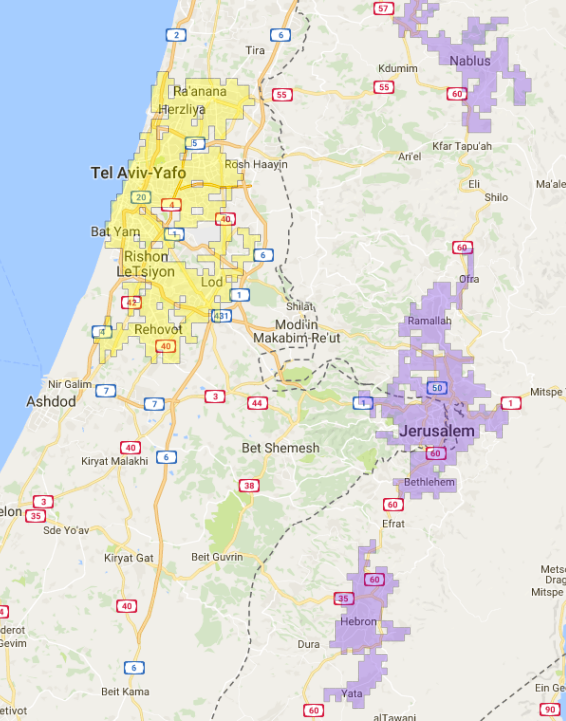
\includegraphics[width=\textwidth]{TelAviv}
  \caption{Geographic Definition of Tel Aviv-Yafo}
   \label{fig:TelAviv}
\end{centering}
\end{figure}
\end{comment}

